!en \section{Get me on, leave me off}
!de \section{Mach' mich an, lass' mich aus}

!en X

!de Zuerst die erweiterte Schaltung

\begin{figure}[htbp]
  \centering
  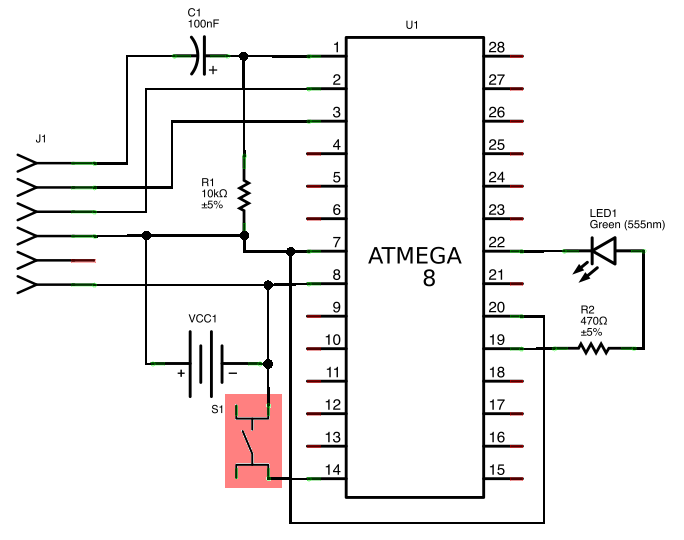
\includegraphics[width=120mm]{LED/S002_get-me-on-get-me-off_Circuit_schema.png}
!en   \caption{Get me on, get me off - Schema}
!de   \caption{Mach' mich an, lass' mich aus - Schaltplan}
  \label{atmega8-get-me-on-get-me-off-schema}
  \label{atmega8-get-me-on-get-me-off-schema}
\end{figure}


!en Second the code

!de Anschliessend das Programm


\begin{lstlisting}
; LED/S002_get-me-on-get-me-off.asm

.DEVICE atmega8

.org 0x0000
            rjmp     start

start:
            sbi     DDRB,         5
            cbi     DDRB,         0
            sbi     PORTB,        0

main:
            sbic    PINB,         0 ; 1 cycles if false or 2
            rjmp    led_on          ; 2 cycles
            cbi     PORTB,        5 ; 1 cycle
            rjmp    led_ok          ; 2 cycles
led_on:
            sbi     PORTB,        5 ; 1 cycle
led_ok:
            rjmp    main            ; 2 cycles
\end{lstlisting}

!en X

!de Wie zu vermuten war, handelt es sich hier bereits ein Programm der 'Zweiten Form'. Es tut nicht nur etwas \textit{vor} der Endlosschleife, sondern ebenfalls etwas darin. Dieses Programm hat wirklich viel zu tun, wie noch sehen werden.



!en X

!de Der erste Unterschied zum vorherigen Programm ist, dass wir ein zusätzliches Bein benutzen, diesmal um ein Eingangssignal zu erkennen. Um dieses Bein, Bit 0 an Port B = Bein 14 am MC, auf den Input Modus zu schalten, senden wir eine \texttt{0} an das entsprechende 'Data Direction Register' (\texttt{DDR}), also \texttt{cbi DDRB, 0}. Ausserdem senden wir eine \texttt{1} auf das Bit am entsprechenden Port, \texttt{sbi PORTB, 1}. Was im Ausgabemodus bedeuten würde 'Schalte VCC an das Bein', heisst im Eingabemodus: 'Schalte den pull-up-Widerstand\footnote{Ein pull-up-Widerstand ist ein Widerstand, der dazu benutzt wird, um den Signalpegel an einem Bein 'hoch' (auf VCC) zu legen = \texttt{1}. Er dient dazu um an einem Eingangsbein auch dann einen stabilen Zustand zu erreichen, wenn kein Element angeschlossen ist.} zu'.



!en X

!de Danach können wir vom Eingangsbein den Status 'EIN' oder '1' lesen. Um eine Reaktion am MC zu erreichen und das Eingangssignal auf 'AUS' oder '0' zu setzen, müssen wir das Beim auf GND ziehen.



!en X

!de Wenn wir das machen, schaltet unser Programm das Licht aus solange wir das Eingangsbein auf Masse legen. Das ist nicht direkt eine Anwendung mit der wir gross angeben können. Für uns ist es dennoch grossartig weil wir verstehen was passiert!



!en If you follow the programs flow:

%de Das Programm läuft folgendermassen ab:

\begin{enumerate}
!en   \item Initialise system and all connected devices
!de   \item Initialisiere das System und die angeschlossenen Geräte
!en   \item (*) Read bit 0
!de   \item (*) Lese Bit 0
!en   \item Set bit 5 accordingly
!de   \item Setze Bit 5 entsprechend
!en   \item Continue with (*)
!de   \item Weiter bei (*)
\end{enumerate}



!en X

!de Jemand, der dieses Programm unter dem Blickwinkel der Sparsamkeit betrachtet, wird sich womöglich fragen, wieso ständig das gleiche Signal auf das Ausgabebit ausgegeben wird. Wenn wir einmal grob annehmen, dass unser Programm das Eingangsbit ca. eine Million mal pro Sekunde liest (eher 8 Mio. mal bei 8MHz ), ist einzusehen, dass ein Mensch mit einem Tasten kaum 'Last' für unseren MC erzeugen kann. Wenn ein Mensch auf den Schalter einhämmert so schnell er kann, passiert aus der Sicht des Micro Controllers so gut wir gar nichts, das Signal ändert sich auf diese Weise für den MC in historischen Zeiträumen.


!en X

!de Die tatsächliche Abfragefrequenz ist möglicher Weise unterschiedlich für die beiden Systemzuständen (Signal \texttt{1} oder \texttt{0}). Wir rechnen kurz nach:

\begin{enumerate}
!en   \item X
!de   \item Signal = '\texttt{1}' entspricht 5 Zyklen
!en   \item X
!de   \item Signal = '\texttt{0}' entspricht 7 Zyklen
\end{enumerate}



!en X

!de Die Schleifendurchlauffrequenz können wir einfach berechnen, indem wir die Taktfrequenz des Prozessors durch die Anzahl der erforderlichen Taktzyklen für einen Schleifendurchlauf teilen.

\begin{equation}
f_{Loop} = \frac{f_{CPU}}{d}
\end{equation}

!en X

!de Wobei d die 'Dauer' eines Schleifendurchlaufs in Zyklen pro Schleifendurchlauf ist. Das bedeutet, dass der MC ohne Druck auf den Taster 8/5 Mio. Mal pro Sekunde den Schaltzustand des Tasters anfragt und bei gedrücktem Taster 8/7 Mio. Mal pro Sekunde.


!en X

!de Solche Abfragefrequenzen sind im Allgemeinen unsinnig. Es gibt Fälle, in denen auch die Bedienung von Tasten durch Menschen zeitkritisch sind, wenn es sich um Musikinstrumente handelt, kommt es auf Millisekunden an. Aber um ein Licht einzuschalten, genügen problemlos 30 Schleifendurchläufe je Sekunde. Mehr kann der Mensch ohnehin nicht erkennen. Kann man das System also optimieren? Wir glauben nicht.



!en X

!de Gibt es andere Lösungen? Ja, die gibt es!



!en \subsection{CPU Frequency}
!de \subsection{CPU Frequenz anpassen}

!en X

!de Wir könnten die Taktfrequenz, mit der die CPU operiert senken. Je nach Einsatzfall kann das tatsächlich helfen, Energie zu sparen, wäre aber damit verbunden, die Rechenleistung des Systems zu reduzieren und kann nachteilig wirken, wenn zusätzliche Aufgaben erledigt werden.



!en X

!de Es kann allerdings nicht schaden, sich in jedem Fall Gedanken über die Taktfrequenzen zu machen, die in einem Micro Controller zusammenkommen. Sowohl nach unten wie auch nach oben. Letztlich beeinflusst eine solche Entscheidung auch die Auswahl des Micro Controllers als solchem.



\subsection{Interrupts}

!en X

!de Vielleicht könnte man auch Interrupts verwenden, um die Signalisierung des Schalterstatus umzukehren. Der Mikroprozessor erledigt dann die Abfrage für uns und signalisiert dem Programm aktiv, dass der Knopf gedrückt wurde. Dieses Verfahren macht einen ruhigeren Eindruck, läuft technisch aber auf das gleiche Prinzip hinaus, mit dem Unterschied, dass wir einen grossen Aufwand zur Initialisierung der Interruptauslösung betreiben müssten, ohne dass die CPU weniger rotieren hätte. Die Hauptprogrammschleife wäre dann leer. Doch sie würde sich auch leer mir dem vollen CPU Takt um sich selbst drehen.



!en X

!de Das heisst, das Programm wird komplizierter - wie wir sehen werden schränkt ein solches Verfahren sogar die Anzahl der Pins ein, die als Schaltereingang benutzt werden können - aber die CPU Last bleibt gleich.


!en X

!de Wirklich nützlich wird dieses Verfahren erst, wenn die CPU abgeschaltet werden könnte, während sie auf einen Interrupt wartet oder - dann sowieso - wenn das Programm parallel noch eine Reihe anderer Aufgaben zu lösen hätte. Beides werden wir noch demonstrieren. Beides ist in der aktuellen Phase aber noch zu komplex.



!en \subsection{X}
!de \subsection{Statusverwaltung}



!en X

!de Wir könnten den zuletzt ausgegebenen Status speichern. Dann könnten wir in der nächsten Programmschleife prüfen ob sich der eingelesene Status zum vorherigen Status geändert hat und nur dann ein Signal an das Bein ausgeben, wenn eine solche Änderung vorliegt. Das könnte uns ersparen, 8/5 oder 8/7 Mio. Mal pro Sekunde den unveränderten Status an die LED auszugeben.



!en X

!de Das klingt gut und einfach, ist es aber leider nicht! Es ist nicht nur nicht einfach, es ist gefährlich, kostspielig und kompliziert. Und es ist effektiv sinnlos weil wir eine Menge Aufwand treiben würden, ohne dass sich wirklich etwas verbessert.



!en X

!de Dieses Konzept ist gefährlich weil das Programm aus dem Rhythmus kommen könnte. Danach würde es falsch herum arbeiten oder überhaupt nicht mehr auf Eingangssignale reagieren.



!en X

!de Es ist kostspielig weil das Programm nicht nur viel grösser würde, wir würden ausserdem ein CPU Register verbrauchen (um den Status zu speichern) und wir haben um \at{} total nur 32 Stück von denen nur die Hälfte einfach zu benutzen ist!



!en X

!de Und es ist kompliziert weil wir zwei unabhängige Einheiten im Gleichlauf halten müssen (das Licht und das Statusregister) um vielleicht einen Effekt zu erzielen. Das ist ein grosses Risiko und ein Nachteil gegenüber der vorliegenden Lösung.



!en X

!de Aus diesen Gründen liegen wir vielleicht nicht falsch mit der Vermutung, dass die Entwickler unseres Micro Controllers ihren Chip so entwickelt haben, dass in Wirklichkeit gar nichts gemacht wird, wenn wir eine '1' auf ein Steuerbit senden, dass bereit auf '1' gesetzt ist. Diese Form der Optimierung darf man erwarten.



!en X

!de In der Summe heisst das, dass wir momentan am Ende unsere Möglichkeiten sind Wir müssen hier also bei der vorliegenden Lösung bleiben. Die Vorgeschlagenen Ansätze werden später allerdings noch aktuell werden.